% Options for packages loaded elsewhere
\PassOptionsToPackage{unicode}{hyperref}
\PassOptionsToPackage{hyphens}{url}
%
\documentclass[
  12pt,
]{article}
\usepackage{amsmath,amssymb}
\usepackage{lmodern}
\usepackage{setspace}
\usepackage{ifxetex,ifluatex}
\ifnum 0\ifxetex 1\fi\ifluatex 1\fi=0 % if pdftex
  \usepackage[T1]{fontenc}
  \usepackage[utf8]{inputenc}
  \usepackage{textcomp} % provide euro and other symbols
\else % if luatex or xetex
  \usepackage{unicode-math}
  \defaultfontfeatures{Scale=MatchLowercase}
  \defaultfontfeatures[\rmfamily]{Ligatures=TeX,Scale=1}
\fi
% Use upquote if available, for straight quotes in verbatim environments
\IfFileExists{upquote.sty}{\usepackage{upquote}}{}
\IfFileExists{microtype.sty}{% use microtype if available
  \usepackage[]{microtype}
  \UseMicrotypeSet[protrusion]{basicmath} % disable protrusion for tt fonts
}{}
\makeatletter
\@ifundefined{KOMAClassName}{% if non-KOMA class
  \IfFileExists{parskip.sty}{%
    \usepackage{parskip}
  }{% else
    \setlength{\parindent}{0pt}
    \setlength{\parskip}{6pt plus 2pt minus 1pt}}
}{% if KOMA class
  \KOMAoptions{parskip=half}}
\makeatother
\usepackage{xcolor}
\IfFileExists{xurl.sty}{\usepackage{xurl}}{} % add URL line breaks if available
\IfFileExists{bookmark.sty}{\usepackage{bookmark}}{\usepackage{hyperref}}
\hypersetup{
  pdftitle={Supporting Information},
  hidelinks,
  pdfcreator={LaTeX via pandoc}}
\urlstyle{same} % disable monospaced font for URLs
\usepackage[margin=1in]{geometry}
\usepackage{longtable,booktabs,array}
\usepackage{calc} % for calculating minipage widths
% Correct order of tables after \paragraph or \subparagraph
\usepackage{etoolbox}
\makeatletter
\patchcmd\longtable{\par}{\if@noskipsec\mbox{}\fi\par}{}{}
\makeatother
% Allow footnotes in longtable head/foot
\IfFileExists{footnotehyper.sty}{\usepackage{footnotehyper}}{\usepackage{footnote}}
\makesavenoteenv{longtable}
\usepackage{graphicx}
\makeatletter
\def\maxwidth{\ifdim\Gin@nat@width>\linewidth\linewidth\else\Gin@nat@width\fi}
\def\maxheight{\ifdim\Gin@nat@height>\textheight\textheight\else\Gin@nat@height\fi}
\makeatother
% Scale images if necessary, so that they will not overflow the page
% margins by default, and it is still possible to overwrite the defaults
% using explicit options in \includegraphics[width, height, ...]{}
\setkeys{Gin}{width=\maxwidth,height=\maxheight,keepaspectratio}
% Set default figure placement to htbp
\makeatletter
\def\fps@figure{htbp}
\makeatother
\setlength{\emergencystretch}{3em} % prevent overfull lines
\providecommand{\tightlist}{%
  \setlength{\itemsep}{0pt}\setlength{\parskip}{0pt}}
\setcounter{secnumdepth}{-\maxdimen} % remove section numbering
\usepackage{geometry}
\geometry{verbose,letterpaper,margin=2.45cm}

% \usepackage[breaklinks=true,pdfstartview=FitH,citecolor=blue]{hyperref}
\hypersetup{colorlinks,%
	citecolor=blue,%
	filecolor=red,%
	linkcolor=blue,%
	urlcolor=red,%
	pdfstartview=FitH}

\usepackage[T1]{fontenc}
\usepackage[utf8]{inputenc}
\usepackage{textgreek}
\usepackage[greek,english]{babel}
\usepackage{microtype}
\usepackage{amsmath}
\usepackage[osf]{libertine}
\usepackage{libertinust1math}
\usepackage{inconsolata}
\usepackage{caption} % to remove figure label with \captionsetup{}

\usepackage{booktabs}

\usepackage{setspace}
\doublespacing

% \setstretch{1.8999999999999999}

\usepackage{lineno}
\linenumbers

\usepackage{lscape}
\newcommand{\blandscape}{\begin{landscape}}
\newcommand{\elandscape}{\end{landscape}}

% \renewcommand{\rmdefault}{cmr}


% flush left while keep identation
\makeatletter
\newcommand\iraggedright{%
  \let\\\@centercr\@rightskip\@flushglue \rightskip\@rightskip
  \leftskip\z@skip}
\makeatother

% make pdf as default figure format
\DeclareGraphicsExtensions{.pdf,.png, %
    .jpg,.mps,.jpeg,.jbig2,.jb2,.JPG,.JPEG,.JBIG2,.JB2}
    
\ifluatex
  \usepackage{selnolig}  % disable illegal ligatures
\fi

\title{Supporting Information}
\author{}
\date{\vspace{-2.5em}}

\begin{document}
\maketitle

% align only at left, not at right.
\iraggedright

% Package command for citing R packages
\newcommand{\pkg}[1]{{\fontseries{b}\selectfont #1}} 

\setstretch{1.5}
\renewcommand\thefigure{S\arabic{figure}}    
\renewcommand\thetable{S\arabic{table}}    
\setcounter{figure}{0}    
\setcounter{table}{0}

\begin{figure}[ht]
  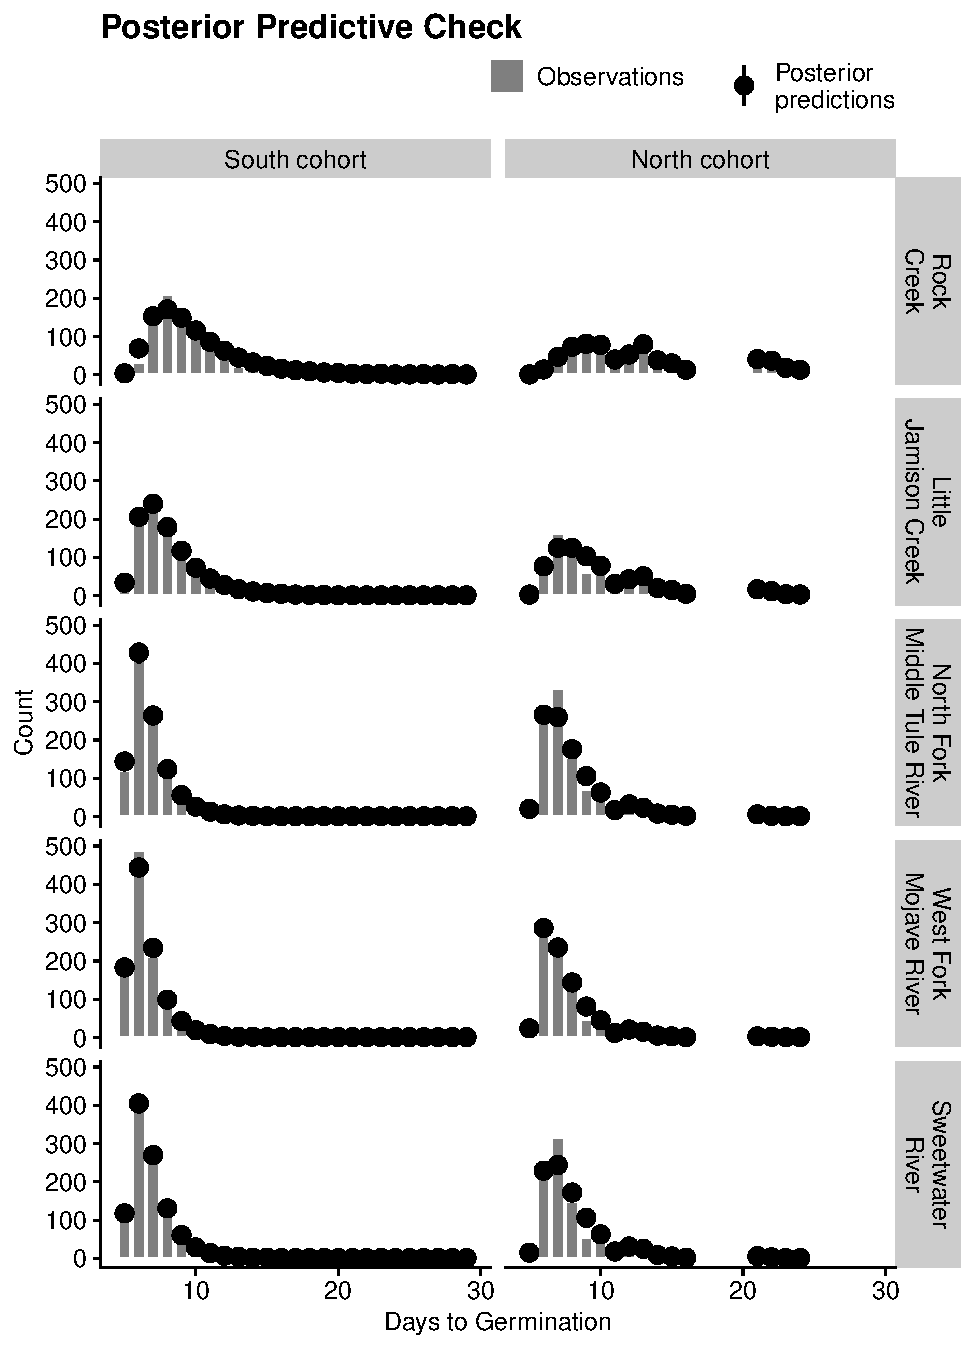
\includegraphics[width=\textwidth]{figures/pp_check_germ.pdf}
  \caption{(Caption next page.)}
  \label{fig:pp_check}
\end{figure}
\addtocounter{figure}{-1}
\begin{figure} [t!]
  \caption{(Previous page.) Posterior predictive check of germination rate from discretized log-normal model for the South cohort (left facets) and North cohort (right facets). Each histogram in gray bars is for one of five \textit{M. cardinalis} populations arranged from northern (top) to southern (bottom). The black points are median values from randomly simulated data sets drawn from each iteration of the posterior distributions. Lines indicate the 95\% confidence interval but are usually too narrow to be seen behind the point estimates. A close match between observations and posterior predictions indicate that the model adequately describes the distribution of the data.}
\end{figure}

\begin{figure}[ht]
  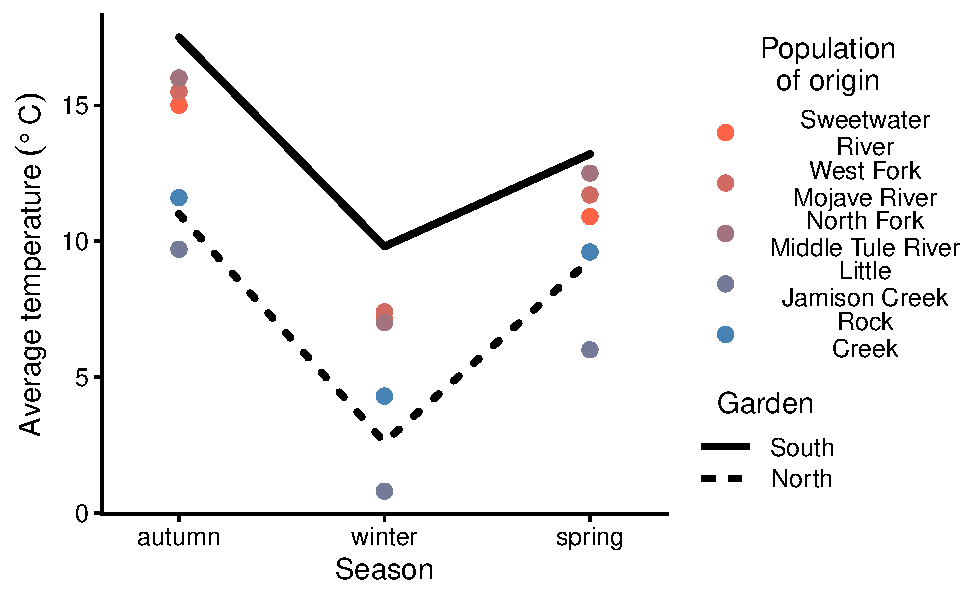
\includegraphics[width=\textwidth]{figures/climate.pdf}
  \caption{The average temperature during the 2015-16 experiment (lines) was warmer than the historical normal from 1961-1990 (points). The $y$-axis is the average temperature for a season in the southern (solid line) and northern (dashed line) garden. Points are the average seasonal temperature for the 1961-1990 normal for each population source location. Population color is arranged from orange to blue by latitude of origin from south to north. Season is along the $x$-axis. Autumn encompasses September-November; winter encompasses December-February; spring encompasses March-May. All down-scaled climate are from ClimateNA (see Materials and Methods).}
  \label{fig:fig:climate}
\end{figure}

\clearpage

\begin{longtable}[]{@{}ll@{}}
\caption{\label{tab:vc_table_germ} We decomposed variance in germination rate among populations (\(V_\text{pop}\)), additive genetic differences among individuals in the base population (\(V_\text{G}\)), experimental blocks within the greenhouse (Block), and residual environmental variance (\(V_\text{E}\)). The narrow-sense heritability \(h^2\) is \(V_\text{G} / (V_\text{G} + V_\text{E})\). Point estimates and 95\% confidence intervals (CI) are estimated from the median and quantiles of the posterior distribution.}\tabularnewline
\toprule
Parameter & Median (95\% CI) \\
\midrule
\endfirsthead
\toprule
Parameter & Median (95\% CI) \\
\midrule
\endhead
\(V_\text{pop}\) & 0.138 (0.0886--0.201) \\
\(V_\text{G}\) & 0.117 (0.0832--0.172) \\
Block & 0.0352 (0.0238--0.0553) \\
\(V_\text{E}\) & 0.266 (0.258--0.275) \\
\(H^2\) & 0.279 (0.213--0.365) \\
\bottomrule
\end{longtable}

\clearpage

\blandscape

\begin{longtable}[]{@{}
  >{\raggedright\arraybackslash}p{(\columnwidth - 6\tabcolsep) * \real{0.27}}
  >{\raggedright\arraybackslash}p{(\columnwidth - 6\tabcolsep) * \real{0.07}}
  >{\raggedright\arraybackslash}p{(\columnwidth - 6\tabcolsep) * \real{0.14}}
  >{\raggedright\arraybackslash}p{(\columnwidth - 6\tabcolsep) * \real{0.52}}@{}}
\caption{\label{tab:vc_table_surv} We decomposed variance in winter survival (\(\text{logit}(p_\text{surv})\)) among populations (\(V_\text{pop}\)), additive genetic differences among individuals in the base population (\(V_\text{G}\)), experimental blocks in the field (Block), and residual environmental variance (\(V_\text{E}\)) for the North and South garden separately. The narrow-sense heritability \(h^2\) is \(V_\text{G} / (V_\text{G} + V_\text{E})\). Point estimates and 95\% confidence intervals (CI) are estimated from the median and quantiles of the posterior distribution.}\tabularnewline
\toprule
Population & Garden & Parameter & Median (95\% CI) \\
\midrule
\endfirsthead
\toprule
Population & Garden & Parameter & Median (95\% CI) \\
\midrule
\endhead
Sweetwater River & North & \(H^2\) & 0.00443 (0.0011--0.0142) \\
Sweetwater River & North & \(V_\text{E}\) & 0.18 (0.147--0.206) \\
Sweetwater River & North & \(V_\text{G}\) & 0.000733 (0.000205--0.00256) \\
Sweetwater River & North & \(V_\text{pop}\) & 0.00757 (0.00379--0.0112) \\
Sweetwater River & North & Block & 0.000733 (0.000205--0.00256) \\
West Fork Mojave River & North & \(H^2\) & 0.00469 (0.00117--0.0157) \\
West Fork Mojave River & North & \(V_\text{E}\) & 0.195 (0.156--0.219) \\
West Fork Mojave River & North & \(V_\text{G}\) & 0.000812 (0.000239--0.0033) \\
West Fork Mojave River & North & \(V_\text{pop}\) & 0.00757 (0.00379--0.0112) \\
West Fork Mojave River & North & Block & 0.000812 (0.000239--0.0033) \\
North Fork Middle Tule River & North & \(H^2\) & 0.00441 (0.0011--0.0141) \\
North Fork Middle Tule River & North & \(V_\text{E}\) & 0.172 (0.138--0.197) \\
North Fork Middle Tule River & North & \(V_\text{G}\) & 0.000675 (0.000198--0.00243) \\
North Fork Middle Tule River & North & \(V_\text{pop}\) & 0.00757 (0.00379--0.0112) \\
North Fork Middle Tule River & North & Block & 0.000675 (0.000198--0.00243) \\
Little Jamison Creek & North & \(H^2\) & 0.00531 (0.00127--0.016) \\
Little Jamison Creek & North & \(V_\text{E}\) & 0.219 (0.18--0.24) \\
Little Jamison Creek & North & \(V_\text{G}\) & 0.00109 (0.000289--0.00348) \\
Little Jamison Creek & North & \(V_\text{pop}\) & 0.00757 (0.00379--0.0112) \\
Little Jamison Creek & North & Block & 0.00109 (0.000289--0.00348) \\
Rock Creek & North & \(H^2\) & 0.00589 (0.00137--0.0186) \\
Rock Creek & North & \(V_\text{E}\) & 0.245 (0.225--0.249) \\
Rock Creek & North & \(V_\text{G}\) & 0.00142 (0.000341--0.00465) \\
Rock Creek & North & \(V_\text{pop}\) & 0.00757 (0.00379--0.0112) \\
Rock Creek & North & Block & 0.00142 (0.000341--0.00465) \\
Sweetwater River & South & \(H^2\) & 0.000937 (\(9.78 \times 10^{-5}\)--0.0043) \\
Sweetwater River & South & \(V_\text{E}\) & 0.0651 (0.0352--0.0998) \\
Sweetwater River & South & \(V_\text{G}\) & 6.5e-05 (\(5.35 \times 10^{-6}\)--0.000405) \\
Sweetwater River & South & \(V_\text{pop}\) & 0.00131 (0.000354--0.00283) \\
Sweetwater River & South & Block & 0.00518 (0.000938--0.0182) \\
West Fork Mojave River & South & \(H^2\) & 0.00102 (0.000104--0.00439) \\
West Fork Mojave River & South & \(V_\text{E}\) & 0.0683 (0.0398--0.106) \\
West Fork Mojave River & South & \(V_\text{G}\) & \(7.75 \times 10^{-5}\) (\(6.87 \times 10^{-6}\)--0.000461) \\
West Fork Mojave River & South & \(V_\text{pop}\) & 0.00131 (0.000354--0.00283) \\
West Fork Mojave River & South & Block & 0.00594 (0.00115--0.0244) \\
North Fork Middle Tule River & South & \(H^2\) & 0.00121 (0.00012--0.00486) \\
North Fork Middle Tule River & South & \(V_\text{E}\) & 0.0794 (0.0483--0.118) \\
North Fork Middle Tule River & South & \(V_\text{G}\) & 0.000105 (\(8.72 \times 10^{-6}\)--0.000634) \\
North Fork Middle Tule River & South & \(V_\text{pop}\) & 0.00131 (0.000354--0.00283) \\
North Fork Middle Tule River & South & Block & 0.00728 (0.0018--0.0269) \\
Little Jamison Creek & South & \(H^2\) & 0.00149 (0.000133--0.00549) \\
Little Jamison Creek & South & \(V_\text{E}\) & 0.088 (0.0512--0.124) \\
Little Jamison Creek & South & \(V_\text{G}\) & 0.000121 (\(1.16 \times 10^{-5}\)--0.000606) \\
Little Jamison Creek & South & \(V_\text{pop}\) & 0.00131 (0.000354--0.00283) \\
Little Jamison Creek & South & Block & 0.0103 (0.00227--0.0315) \\
Rock Creek & South & \(H^2\) & 0.00208 (0.00021--0.00792) \\
Rock Creek & South & \(V_\text{E}\) & 0.129 (0.0818--0.155) \\
Rock Creek & South & \(V_\text{G}\) & 0.000303 (\(3.09 \times 10^{-5}\)--0.00117) \\
Rock Creek & South & \(V_\text{pop}\) & 0.00131 (0.000354--0.00283) \\
Rock Creek & South & Block & 0.0208 (0.00488--0.05) \\
\bottomrule
\end{longtable}

\elandscape

\clearpage

\begin{longtable}[]{@{}lll@{}}
\caption{\label{tab:df_pop_lm} Between-population directional selection coefficient estimates and confidence intervals. In both North and South gardens, we estimated selection on increased germination rate (log-mean scale) caused by increased winter survival (\(\text{logit}(p_\text{surv})\)). The parameters are the linear regression slope and intercept. Point estimates and 95\% confidence intervals (CI) are estimated from the median and quantiles of the posterior distribution.}\tabularnewline
\toprule
Garden & Parameter & Median (95\% CI) \\
\midrule
\endfirsthead
\toprule
Garden & Parameter & Median (95\% CI) \\
\midrule
\endhead
North & intercept & 4.05 (3.09 -- 5.32) \\
North & slope & -0.455 (-0.642 -- -0.328) \\
South & intercept & 4.87 (3.82 -- 6.1) \\
South & slope & -0.354 (-0.528 -- -0.221) \\
\bottomrule
\end{longtable}

\begin{longtable}[]{@{}lll@{}}
\caption{\label{tab:df_ind_lm} Genotypic directional selection coefficient estimates and confidence intervals. In both North and South gardens, we estimated selection on increased germination rate (log-mean scale) caused by increased winter survival (\(\text{logit}(p_\text{surv})\)). The parameters are the linear regression slope and intercept. Point estimates and 95\% confidence intervals (CI) are estimated from the median and quantiles of the posterior distribution.}\tabularnewline
\toprule
Garden & Parameter & Median (95\% CI) \\
\midrule
\endfirsthead
\toprule
Garden & Parameter & Median (95\% CI) \\
\midrule
\endhead
North & intercept & -0.00157 (-0.0349 -- 0.0273) \\
North & slope & -0.13 (-0.374 -- 0.0133) \\
South & intercept & 0.000634 (-0.0173 -- 0.0257) \\
South & slope & -0.00276 (-0.15 -- 0.138) \\
\bottomrule
\end{longtable}

\clearpage

\end{document}
